% !TeX spellcheck = en_US
\documentclass[11pt]{article}

\usepackage[hmargin=2.8cm,vmargin=2.4cm]{geometry}
\usepackage{mathtools}
\usepackage[dvipsnames]{xcolor}
\usepackage{amssymb,dsfont,stmaryrd}
\usepackage{algorithm2e}
\usepackage{hyperref,cleveref}
\usepackage{graphicx}
\usepackage{booktabs}
\usepackage{subcaption}
\usepackage{enumitem}
\usepackage[noindentafter]{titlesec}
\usepackage{tikz}

\usetikzlibrary{bayesnet,arrows,backgrounds}


\setlist{itemsep=0pt}

\hypersetup{
	urlcolor=NavyBlue
}

%%% Math macros %%%

\newcommand\RR{\mathbb{R}}
\newcommand\CC{\mathbb{C}}
\newcommand\ZZ{\mathbb{Z}}
\newcommand\NN{\mathbb{N}}
\newcommand\TT{\mathbb{T}}
\newcommand\PP{\mathbb{P}}
\newcommand\EE{\mathbb{E}}
\newcommand\VV{\mathbb{V}}
\DeclarePairedDelimiter{\intinterv}{\llbracket}{\rrbracket}

\renewcommand{\epsilon}{\varepsilon}

\newcommand{\suchthat}{\mathrm{s.t.}}

\DeclareMathOperator*{\argmin}{\mathrm{argmin}}
\DeclareMathOperator*{\argmax}{\mathrm{argmax}}
\DeclareMathOperator{\diag}{\mathrm{diag}}
\DeclareMathOperator{\sgn}{\mathrm{sgn}}
\DeclareMathOperator{\trace}{\mathrm{Tr}}

\newcommand{\calM}{\mathcal{M}}
\newcommand{\calP}{\mathcal{P}}
\newcommand{\calN}{\mathcal{N}}
\newcommand{\calX}{\mathcal{X}}
\newcommand{\calL}{\mathcal{L}}
\newcommand{\calC}{\mathcal{C}}
\newcommand{\calD}{\mathcal{D}}

\newcommand{\bmmu}{\boldsymbol{\mu}}
\newcommand{\bmpsi}{\boldsymbol{\psi}}
\newcommand{\bmphi}{\boldsymbol{\phi}}

\newcommand{\bmX}{\boldsymbol{X}}

\colorlet{darkblue}{RoyalBlue!90!black}
\colorlet{darkred}{Red!95!black}
\newcommand{\bluefont}{\color{darkblue}}
\newcommand{\redfont}{\color{darkred}}


%%% Section titling setup %%%

\titleformat*{\section}{\LARGE\bfseries\sffamily}
\titleformat*{\subsection}{\Large\bfseries\sffamily}

\titleformat{\paragraph}[hang]{\sffamily\large\bfseries}{}{}{}[]

\titleformat{\subparagraph}[runin]{\sffamily\bfseries}{}{}{\textbullet}[]

% \titlespacing{command}{left}{before-sep}{after-sep}
\titlespacing*{\subparagraph}{2pt}{*2}{*1.5}

%%% Document title %%%

\title{
	MVA -- Probabilistic Graphical Models\\
	{\color{NavyBlue}\sffamily Homework 3: Gibbs Sampling and VB}
}

\author{
	Wilson \textsc{Jallet}\thanks{\url{wilson.jallet@polytechnique.org}}}


\begin{document}

\maketitle


\paragraph{Question 1}
This operation puts all the data on the same scale -- this is especially useful because the prior on $\beta$ assigns the same variance in each direction.


\paragraph{Question 2}
If we supposed that $\epsilon_i$ had a variance of $\sigma^2$, we could write $\epsilon_i = \sigma \epsilon'_i$ where $\epsilon'_i \sim \calN(0,1)$, and we'd have
\[
	y_i = \sgn(\beta^T x_i + \epsilon_i) =
	\sgn({\beta'}^T x_i + \epsilon'_i)
\]
where $\beta' = \beta/\sigma$.


\paragraph{Question 3}
We define the following graphical model:
\begin{itemize}
	\item observed features $x_i \in \RR^p$, $i\in\{1,\ldots,n\}$
	\item random variable $\beta\sim \calN(0, \tau I_p)$
	\item latent variables $z_i = \beta^Tx_i + \epsilon_i$, $\epsilon_i \sim \calN(0,1)$
	\item observed labels $y_i = \sgn(z_i) \in \{-1,1\}$
\end{itemize}
It has the following representation:
\begin{figure}[h]
	\centering
	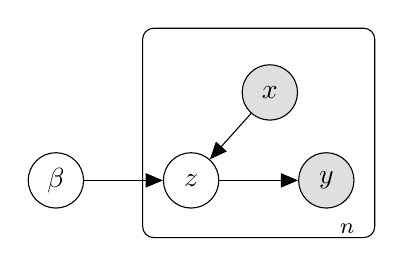
\begin{tikzpicture}
	\node[obs] (y) {$y$};%
	\node[latent,left=of y] (z) {$z$}; %
	\node[latent,left=of z] (beta) {$\beta$}; %
	\node[obs,above=of z,xshift=10mm,yshift=-6mm] (x) {$x$};
	% plate
	\plate [inner sep=.25cm,yshift=.2cm] {plate1} {(x)(y)(z)} {$n$}; %
	% edges
	
	\edge {x} {z};
	\edge {z} {y};
	\edge {beta} {z};
	
	\end{tikzpicture}
\end{figure}

To perform inference on the model, we need the posterior distribution of $\beta, z$ given the data $X,y$.

Our first approach is to use Gibbs sampling. To use it, we need to derive the conditional posteriors of the variables.
Evidently,
\begin{align*}
	p(y_i|\beta)
	= \Phi(y_i\beta^Tx_i)  \\
	p(z_i | \beta)  \sim \calN(\beta^T x_i, 1)  \\
	p(y_i,z_i|\beta) = \mathds{1}_{\{y_iz_i > 0\}}
\end{align*}
By Bayes' theorem we have the posteriors
\begin{equation}
\begin{aligned}
	p(\beta|z) \propto p(\beta)p(z|\beta)
	&\propto \exp\left(
		-\frac1{2\tau}\|\beta\|^2
		-\frac{1}{2}\sum_{i=1}^{n}(z_i - \beta^T x_i)^2
	\right)  \\
	&= \exp\left(
		-\frac1{2\tau}\|\beta\|^2
		-\frac{1}{2}\|z - X\beta\|^2
	\right)
\end{aligned}
\end{equation}
and
\begin{equation}
	p(z|\beta,y) \propto p(z|\beta)p(y,z|\beta)
	\propto \exp\left(
	-\frac{1}{2}\|z - X\beta\|^2
	\right) \prod_{i=1}^{n} \mathds{1}_{\{y_iz_i > 0\}}
\end{equation}
where $X = (x_1|\ldots|x_n)^T \in \RR^{n \times p}$ is the design matrix. By identification $\beta|z \sim \calN(\mu_p, \Sigma_p)$ where
\begin{equation}\label{eq:BetaPostZ}
\bluefont
	\Sigma_p^{-1} = \frac{1}{\tau}I_p + X^TX,
	\quad
	\mu_p = \Sigma_p X^Tz
\end{equation}
and for all $i$, $\boxed{z_i|\beta,y_i \sim \mathrm{T}\calN(x_i^T\beta, 1; y_i)}$ where $\mathrm{T}\calN(\cdot; y_i)$ is the truncated Gaussian with support in the orthant $\{z\in\RR: y_iz_i > 0\}$.

With all this in place, we use Gibbs sampling to sample from the posterior distribution of $\beta,z$ given the data $(X,y)$.
For inference and testing, we \textbf{\boldmath split the dataset up as $2/3$rds for training and $1/3$rd for testing}. \Cref{fig:GibbsMarginals} shows approximate posterior marginals for $\beta,z | X,y$ in the form of histograms made from samples.

The testing accuracy (predicting using MAP) is of about $\approx 75\%$, using 4000 samples of $\beta|X_\mathrm{train},y_\mathrm{train}$.

\begin{figure}
	\centering
	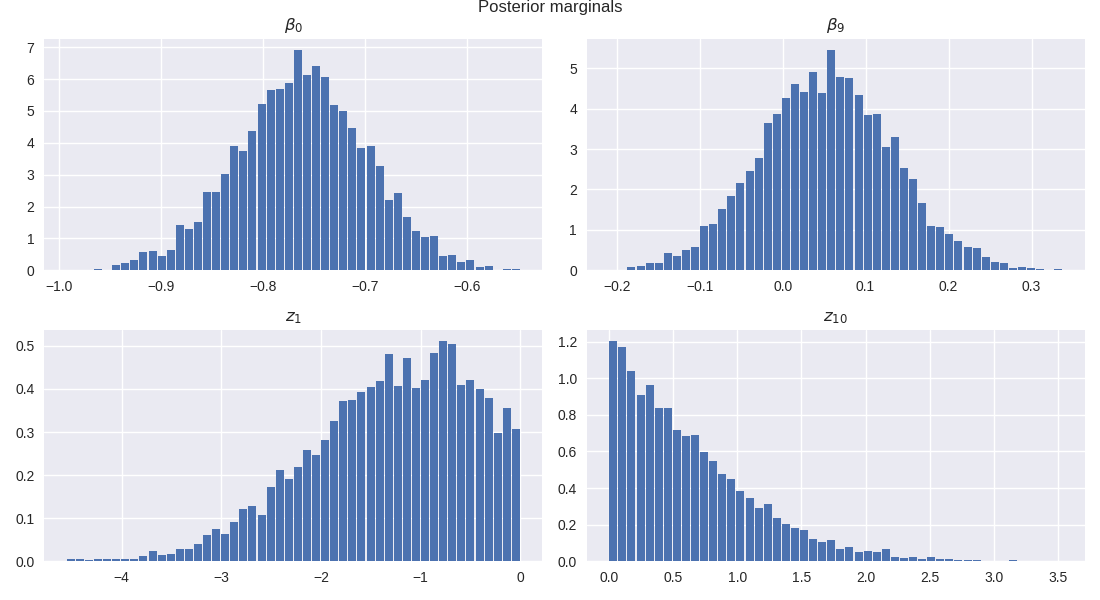
\includegraphics[width=.9\linewidth]{images/posterior_distribution_gibbs.png}
	\caption{Some approximate posterior marginals for $\beta$ and $z$ given the data $X, y$.}\label{fig:GibbsMarginals}
\end{figure}


\paragraph{Question 4}

This time, we want to use variational inference, by approximating the true prior $p(\beta,z|X,y)$ by a distribution $q(\beta,z)$.
Assume the mean-field factorization for $q$:
\begin{equation}
	q(\beta, z) = q_1(\beta)q_2(z)
\end{equation}
We denote by $\EE^q$ the expectation operator under the distribution $q$. The optimal variational distribution satisfies
\begin{subequations}
\begin{align}
	\log q^*_1(\beta) &= \EE_{z\sim q^*_2}[\log p(\beta,z,y)|\beta,y] + \mathrm{cst}  \\
	\log q^*_2(z) &= \EE_{\beta\sim q^*_1}[\log p(\beta,z,y)|z,y] + \mathrm{cst}
\end{align}
\end{subequations}

\subparagraph{Joint probability.} The log-joint probability of $(\beta,z,y)$ is written
\begin{equation}
\begin{aligned}
	\log p(\beta, z, y)
	&= \log p(y | z) + \log p(z|\beta) + \log p(\beta)  \\
	&= 
	\log p(y|z)
	-\frac{1}{2}\|z-X\beta\|^2 - \frac{1}{2\tau} \|\beta\|^2 + \mathrm{cst}
\end{aligned}
\end{equation}

\subparagraph{Derivation of \boldmath$q_1$.} The optimal form of the factor is
\begin{equation}
\begin{aligned}
	\log q^*_1(\beta) &= \EE^{q}_{z}\left[
		\log p(y|z) - \frac{1}{2}\|z-X\beta\|^2 - \frac{1}{2\tau} \|\beta\|^2
		\middle| \beta,y
	\right] + C_1  \\
	&= \EE^q_z [\log p(y|z) | \beta,y]
	- \frac{1}{2} \EE^q_z\left[\|z-X\beta\|^2 \middle| \beta,y\right]
	- \frac{1}{2\tau}\|\beta\|^2
	+ C_1  \\
	&= -\frac{1}{2} \EE^q_z\left[\|z-X\beta\|^2 \middle| \beta,y\right]
	- \frac{1}{2\tau}\|\beta\|^2
	+ C_2  \\
	&= -\frac{1}{2} \EE^q_z\left[\|z\|^2 - 2z^TX\beta + \|X\beta\|^2 \middle| \beta,y\right]
	- \frac{1}{2\tau}\|\beta\|^2
	+ C_2  \\
	&=
	\bar{z}^TX\beta
	-\frac{1}{2}\beta^TX^TX\beta
	-\frac{1}{2\tau}\|\beta\|^2
	+ C_3  \\
	&=
	-\frac{1}{2}
	(\beta - \bar{\beta})\Sigma_p^{-1}(\beta - \bar{\beta})
	+ C_3  \\
\end{aligned}
\end{equation}
where $\Sigma_p$ is defined as in \cref{eq:BetaPostZ}, and
\begin{equation}\label{eq:VBayesParams}
{\redfont
	\bar{z} = \EE_{z\sim q^*_2}[z], \quad
	\bar{\beta} = \Sigma_p X^T\bar{z}.
}
\end{equation}
The terms $\EE^q_z[\log p(y|z)|\beta,y]$ and $\EE^q_z\left[\|z\|^2\right]$ do not depend on $\beta$ and are added to the constants.

The end result is
\begin{equation}
\bluefont
\boxed{
	q^*_1(\beta) = \calN(\Sigma_pX^T {\redfont\bar{z}}, \Sigma_p).
}
\end{equation}


\subparagraph{Derivation of \boldmath$q_2$.} The optimal form of the factor is
\begin{equation}
\begin{aligned}
	\log q^*_2(z)
	&= \EE_{\beta\sim q^*_1}\left[
	\log p(y|z) - \frac{1}{2}\|z-X\beta\|^2 - \frac{1}{2\tau} \|\beta\|^2
	\middle| z,y
	\right] + C_1  \\
	&=
	\sum_{i=1}^n \left\{ 
		\mathds{1}_{y_i=1}\ln(\mathds{1}_{z_i > 0}) + \mathds{1}_{y_i=-1}\ln(\mathds{1}_{z_i \leq 0})
	\right\}
	-\frac{1}{2}
	\left(
		\|z\|^2 - 2z^TX\bar{\beta}
	\right)
	+ C_2  \\
	&=
	\sum_{i=1}^n \left\{ 
	\mathds{1}_{y_i=1}\ln(\mathds{1}_{z_i > 0}) + \mathds{1}_{y_i=-1}\ln(\mathds{1}_{z_i \leq 0})
	\right\}
	-\frac{1}{2}
	\left\|z - X\bar{\beta}\right\|^2
	+ C_3
\end{aligned}
\end{equation}
where $\redfont\bar{\beta} = \EE_{\beta\sim q^*_1}[\beta]$.
Indeed, the expectation under $q_1$ of $\log p(y|z)$ conditionally on $z,y$ is itself.
This means that 
\begin{equation}
\bluefont
\boxed{
	q^*_2(z) = \mathrm{T}\calN(X {\redfont\bar{\beta}}, I_p; \calP_y).
}
\end{equation}




\subparagraph{Summary and algorithm.} The optimal mean-field distribution $q(\beta,z) = q_1(\beta)q_2(z)$ satisfies the fixed-point condition
\begin{subequations}\label{eq:VBfixedPoint}
\begin{align}
	q_1^*(\beta) &= \calN(\Sigma_pX^T\bar{z}, \Sigma_p)  \\
	q_2^*(z) &= \mathrm{T}\calN(X\bar{\beta}, I_p; \calP_y)  \\
	\bar{\beta} &= \EE_{\beta \sim q^*_1}[\beta] = \Sigma_p X^T\bar{z}  \\
	\bar{z} &= \EE_{z \sim q^*_2}[z]
\end{align}
\end{subequations}
We can explicitly compute
\[
	\bar{z}_i = x_i^T\bar{\beta} + y_i\frac{\phi(x_i^T\bar\beta)}{\Phi(y_i x_i^T\bar\beta)}.
\]
The coordinate ascent variational approximation algorithm now reduces to alternatively updating the means until convergence.


\begin{figure}
	\centering
	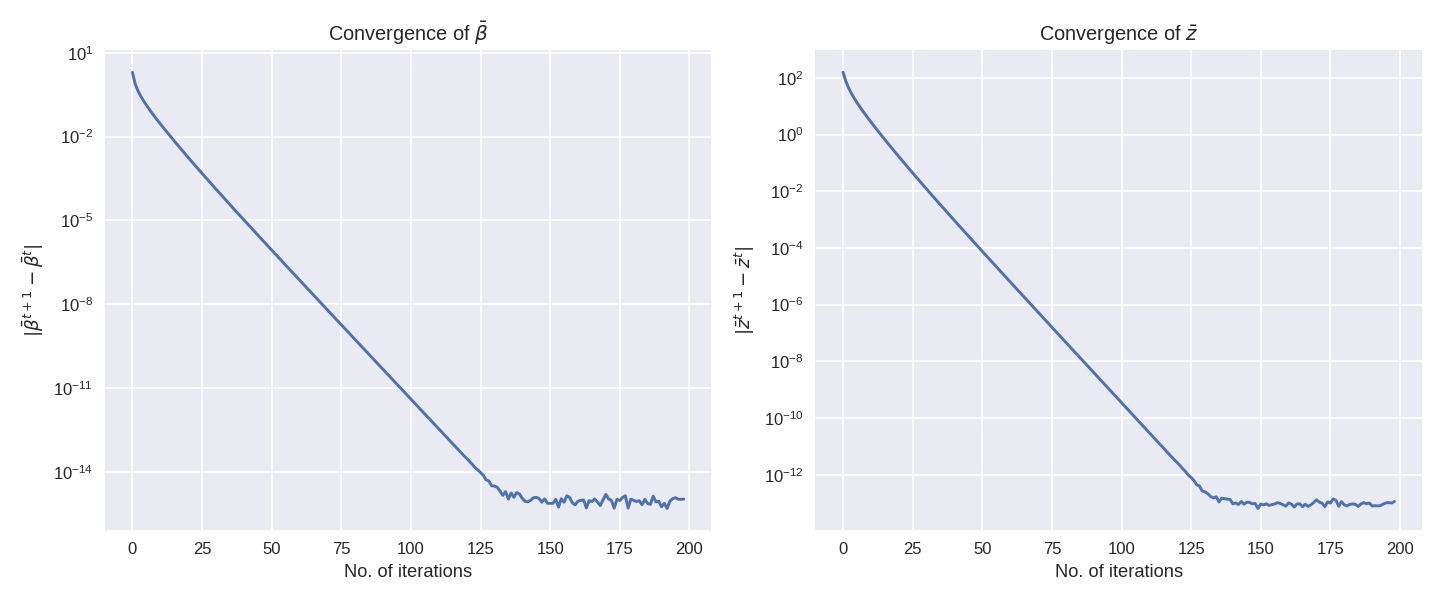
\includegraphics[width=\linewidth]{images/VI_mean_convergence.png}
	\caption{$L_1$-loss between consecutive iterations of the VI algorithm.}\label{fig:VI_L1_convergence}
\end{figure}

\subparagraph{Performance.} Inference with Gibbs sampling $M=5000$ samples (and a burn-in of 100) takes $\approx 10.4$ seconds. Variational approximation converges in 200 iterations (see \cref{fig:VI_L1_convergence}) in $\approx 0.22$ seconds, and sampling $M=5000$ times took $\approx 0.26$ seconds. \Cref{fig:VBGibbsPosteriorComparison} shows a comparison of the posterior marginals obtained with the two approaches: we can observe that the VI algorithm often returns lower posterior variance on $\beta$ than Gibbs. For prediction, we obtain similar MAP prediction accuracy on the test set -- around $75\%$.

\begin{figure}[h]
	\centering
	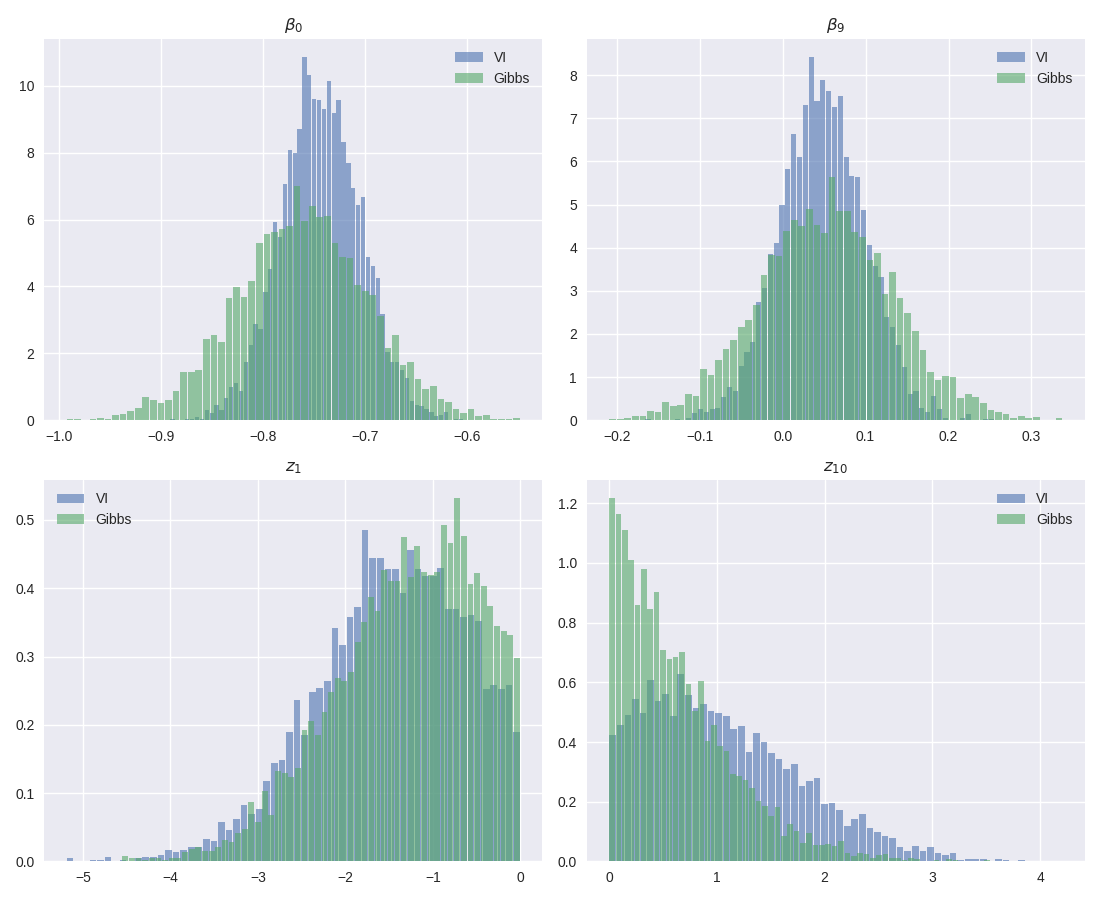
\includegraphics[width=.75\linewidth]{images/posterior_VI_Gibbs_comparison_1.png}
	\caption{Comparison of the posterior marginals between Variational Bayes and Gibbs sampling. Histograms built with $M=5000$ samples.}\label{fig:VBGibbsPosteriorComparison}
\end{figure}

\paragraph{Question 5} We know that the (true) posterior variance of $\beta$ given $X$ is by the law of total variance
\[
	\VV(\beta) = \EE[\VV(\beta|z)] + \VV(\EE[\beta|z]) = \Sigma_p + \VV(\Sigma_pX^Tz) = \Sigma_p + \Sigma_pX\VV(z)X^T\Sigma_p \succeq \Sigma_p
\]
while under $q^*_1$, $\beta$ exactly has variance $\Sigma_p$. So we know that asymptotically VB under-estimates the true posterior variance. It also has lesser variance than the Gibbs iterates $\beta^{(t)}$ by using the same of argument total variance:
\[
	\VV(\beta^{(t)}) = \Sigma_p + \VV(\Sigma_p X^Tz^{(t-1)})
\]


\paragraph{Question 6}


\Cref{fig:CompleteSeparDataset} shows a completely separated dataset in $\RR^2$ -- the separation line $x_1 + 1.5x_2 + 0.1 > 0$ is supported by a normal vector $\beta_\mathrm{true} = (1, 1.5)^T$, and bias $0.1$. A logistic regression model with maximum likelihood estimation would break down and not converge.

For this dataset, the Gibbs sampler might not converge: if we have bias (an additional column in $X$ with ones), we get the trace plot of \Cref{fig:CompleteSeparFailedConv}.

If we introduce instead a smaller constant column (of value $c = 10^{-3}$), we get \Cref{fig:CompleteSeparSmallBiasFix} where we can see the trace plot converge fast and that the posterior histograms resemble actual normal distributions.
This is the same thing as introducing a different, much higher \textit{prior} for the bias variable, which in the supervised regression setting is equivalent to introducing penalization for the bias. This is still not perfect, as we can see in the histogram that the posterior distribution of $\beta_0$ lies in the range $\sim 400-600$: the corresponding bias (renormalizing by $c$) is estimated to be in $\sim 0.4-0.6$, which is wrong. In this setting MAP prediction accuracy on a test set of $1/5$th of the total data yields an accuracy of $89.5\%$.


\begin{figure}[h]
	\centering
	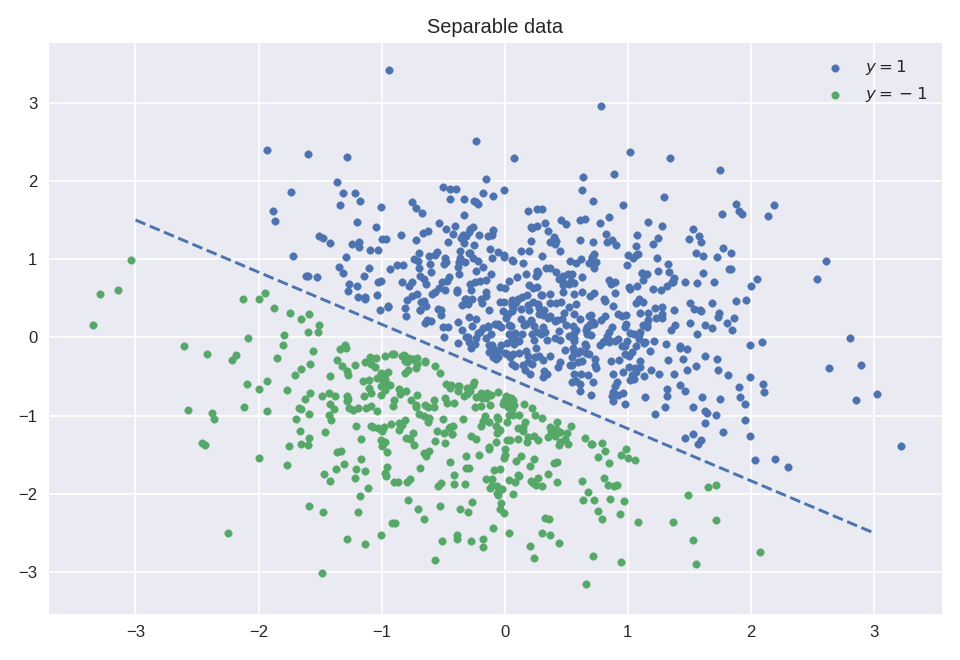
\includegraphics[width=.66\linewidth]{images/separable_data.png}
	\caption{Linearly separable data in dimension $p=2$.}\label{fig:CompleteSeparDataset}
\end{figure}

\begin{figure}
	\centering
	\begin{subfigure}[t]{.66\linewidth}
	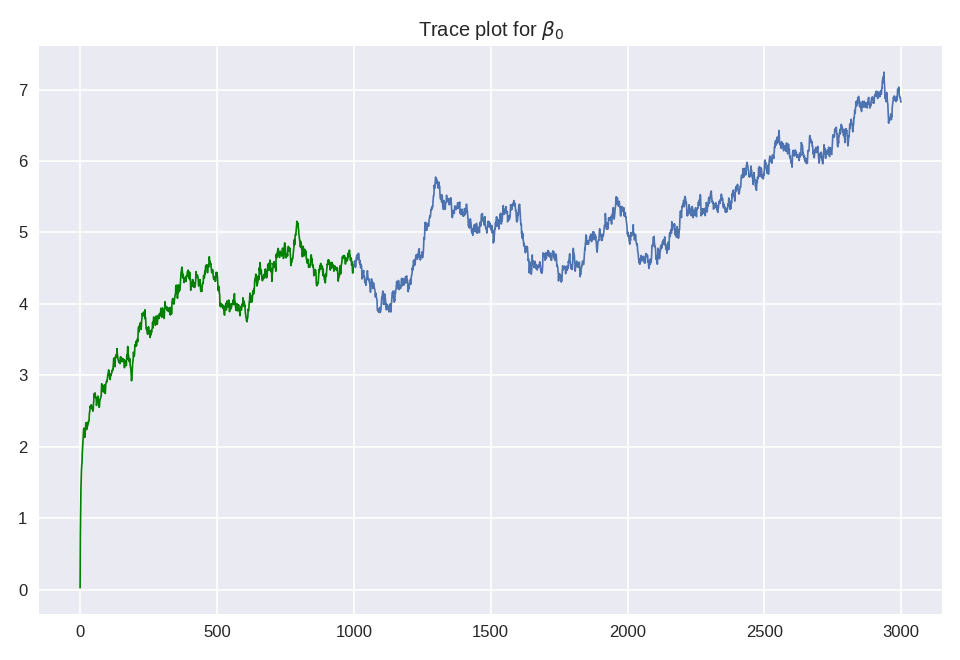
\includegraphics[width=\linewidth]{images/separable_traceplot_fail.png}
	\caption{Trace plot of $\beta_0$.}	
	\end{subfigure}
	\begin{subfigure}[t]{.66\linewidth}
	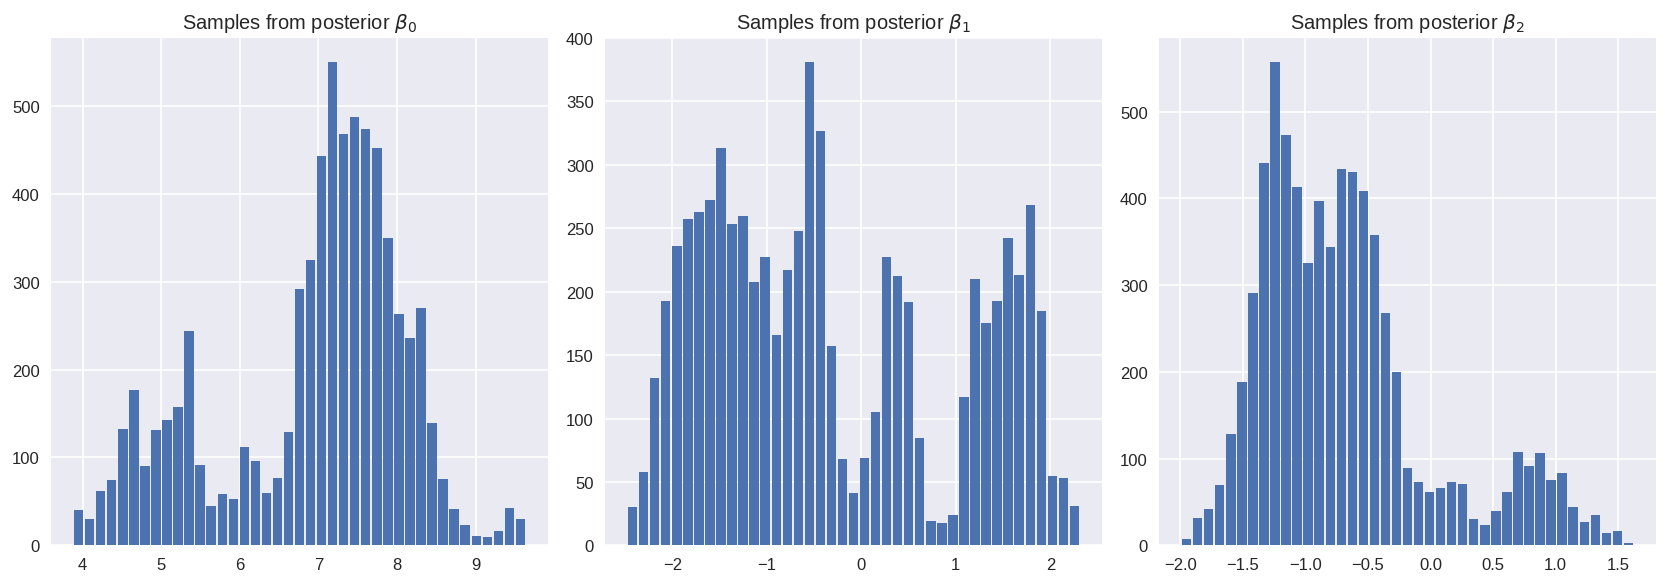
\includegraphics[width=\linewidth]{images/separable_fail_posteriorhist.png}
	\caption{Histogram of the posterior $\beta$ marginals.}	
	\end{subfigure}
	\caption{Failed convergence of Gibbs sampling for the separable dataset when a bias term is added. Increasing the amount of burn-in does not solve the problem.}\label{fig:CompleteSeparFailedConv}
\end{figure}

\begin{figure}
	\centering
	\begin{subfigure}[t]{.66\linewidth}
	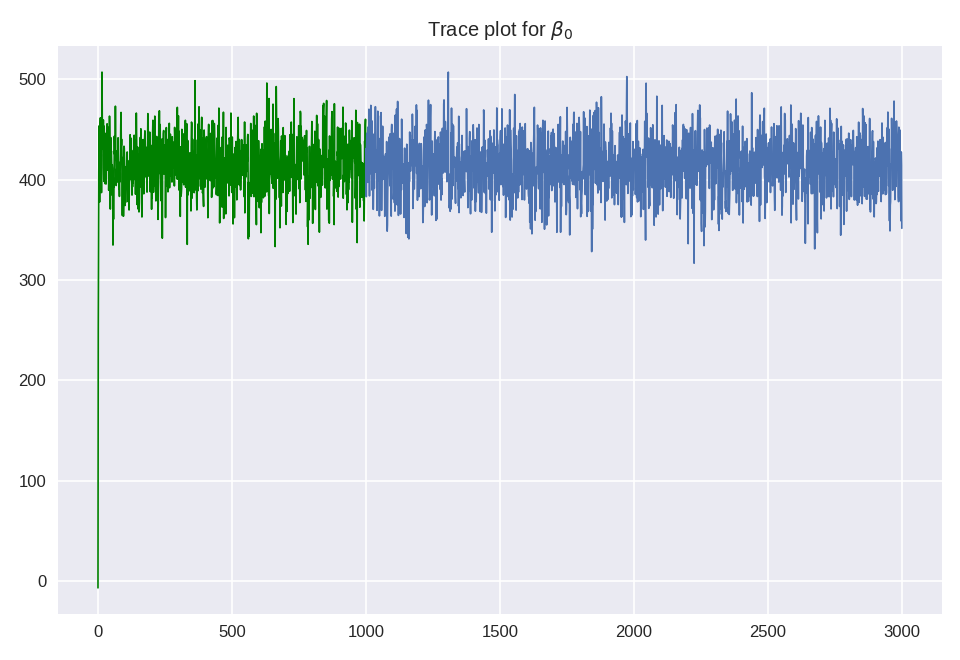
\includegraphics[width=\linewidth]{images/separable_smallbias_trace.png}
	\caption{Trace plot.}
	\end{subfigure}
	\begin{subfigure}[t]{.66\linewidth}
	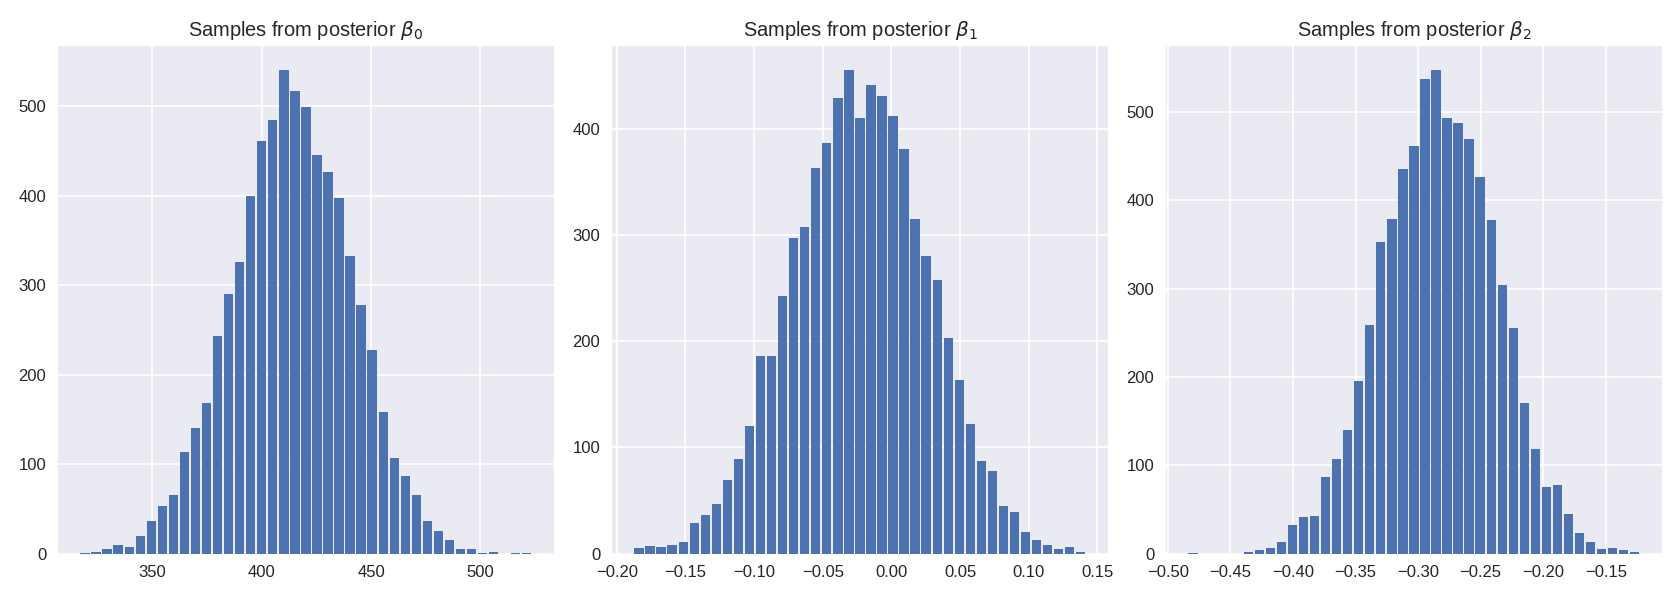
\includegraphics[width=\linewidth]{images/separable_smallbias_posteriorhist.png}
	\caption{Histograms of the posterior $\beta$ marginals.}
	\end{subfigure}
	\caption{Gibbs sampling. Trace plot and posterior $\beta$ histograms using a smaller constant column for the separable data of \cref{fig:CompleteSeparDataset}.}\label{fig:CompleteSeparSmallBiasFix}
\end{figure}



\end{document}
